\documentclass{article}
\usepackage{graphicx}
\graphicspath{{images/}}
\begin{document}
\noindent Adam Frazee \\
Homework 6 \\
10/22/2105 \\
CSE 278 \\

\noindent \textbf{B.11} [5] <4.2, B.2, B.3> Assume that X consists of 3 bits, x2 x1 x0. Write four logic functions that are true if and only if 
\begin{itemize}
	\item X contains only one 0 \\
	$F=\overline{x}_2 \cdot x_1 \cdot x_0 + x_2 \cdot \overline{x}_1 \cdot x_0 + x_2 \cdot x_1 \cdot \overline{x}_0$
	\\ \begin{tabular}{|c|c|c|c|}
	\hline
	$x_2$ & $x_1$ & $x_0$ & result \\ \hline
	0 & 0 & 0 & 0 \\ \hline
	0 & 0 & 1 & 0 \\ \hline
	0 & 1 & 0 & 0 \\ \hline
	0 & 1 & 1 & 1 \\ \hline
	1 & 0 & 0 & 0 \\ \hline
	1 & 0 & 1 & 1 \\ \hline
	1 & 1 & 0 & 1 \\ \hline
	1 & 1 & 1 & 0 \\ \hline
	\end{tabular}
	\item X contains an  even number of 0s \\
		$F=\overline{x}_2 \cdot \overline{x}_1 \cdot x_0 + x_2 \cdot \overline{x}_1 \cdot x_0 + \overline{x}_2 \cdot x_1 \cdot x_0+ x_2 \cdot x_1 \cdot x_0$
	\\ \begin{tabular}{|c|c|c|c|}
	\hline
	$x_2$ & $x_1$ & $x_0$ & result \\ \hline
	0 & 0 & 0 & 0 \\ \hline
	0 & 0 & 1 & 1 \\ \hline
	0 & 1 & 0 & 1 \\ \hline
	0 & 1 & 1 & 0 \\ \hline
	1 & 0 & 0 & 1 \\ \hline
	1 & 0 & 1 & 0 \\ \hline
	1 & 1 & 0 & 0 \\ \hline
	1 & 1 & 1 & 1 \\ \hline
	\end{tabular}
	\item  X when interpreted as an unsigned binary number is less than \\
		$F=\overline{x}_2$
	\\ \begin{tabular}{|c|c|c|c|}
	\hline
	$x_2$ & $x_1$ & $x_0$ & result \\ \hline
	0 & 0 & 0 & 1 \\ \hline
	0 & 0 & 1 & 1 \\ \hline
	0 & 1 & 0 & 1 \\ \hline
	0 & 1 & 1 & 1 \\ \hline
	1 & 0 & 0 & 0 \\ \hline
	1 & 0 & 1 & 0 \\ \hline
	1 & 1 & 0 & 0 \\ \hline
	1 & 1 & 1 & 0 \\ \hline
	\end{tabular} 
	\pagebreak
	\item X when interpreted as a signed (two’s complement) number is 
negative\\
		$F=x_2$
	\\ \begin{tabular}{|c|c|c|c|}
	\hline
	$x_2$ & $x_1$ & $x_0$ & result \\ \hline
	0 & 0 & 0 & 0 \\ \hline
	0 & 0 & 1 & 0 \\ \hline
	0 & 1 & 0 & 0 \\ \hline
	0 & 1 & 1 & 0 \\ \hline
	1 & 0 & 0 & 1 \\ \hline
	1 & 0 & 1 & 1 \\ \hline
	1 & 1 & 0 & 1 \\ \hline
	1 & 1 & 1 & 1 \\ \hline
	\end{tabular} 
\end{itemize}
\noindent \textbf{B.14} [5] <§§B.2, B.3>Implement a switching network that has two data inputs (A and B), two data outputs (C and D), and a control input (S). If S equals 1, the network is in pass-through mode, and C should equal A, and D should equal B. If S equals 0, the network is in crossing mode, and C should equal B, and D should
equal A. 

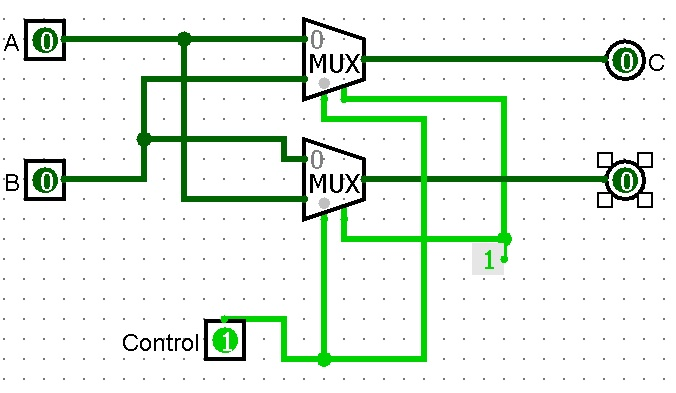
\includegraphics{logsim}
\end{document}